%----------------------ELEMENTOS PÓS-TEXTUAIS----------------------%
\postextual

%--------------------Referências Bibliográficas--------------------%
\bibliography{bibliografia}


%-----------------------------Apêndices-----------------------------%
\begin{apendicesenv}

\chapter{Tutorial Básico de \LaTeX}

\section*{Introdução}
\LaTeX{} é um sistema de preparação de documentos de alta qualidade tipográfica, amplamente utilizado em publicações científicas e acadêmicas. Este tutorial oferece uma introdução detalhada ao \LaTeX, cobrindo os conceitos e comandos fundamentais para a criação de documentos profissionais.

\section*{Estrutura Básica de um Documento}
Um documento \LaTeX{} típico possui a seguinte estrutura básica:

\begin{verbatim}
\documentclass{classe}
\usepackage{pacotes}

\begin{document}
    % Conteúdo do documento
\end{document}
\end{verbatim}

\begin{itemize}
    \item \texttt{\textbackslash documentclass\{classe\}}: Define a classe do documento (e.g., \texttt{article}, \texttt{report}, \texttt{book}).
    \item \texttt{\textbackslash usepackage\{pacotes\}}: Inclui pacotes adicionais para funcionalidades extras.
    \item \texttt{\textbackslash begin\{document\}} e \texttt{\textbackslash end\{document\}}: Delimitam o início e o fim do conteúdo do documento.
\end{itemize}

\section*{Texto e Formatação}
Você pode escrever texto normalmente e utilizar comandos para formatação. Alguns exemplos:

\subsection*{Negrito e Itálico}
\begin{itemize}
    \item \texttt{\textbackslash textbf\{texto\}}: \textbf{texto em negrito}
    \item \texttt{\textbackslash textit\{texto\}}: \textit{texto em itálico}
\end{itemize}

\subsection*{Listas}
\LaTeX{} permite criar listas numeradas e não numeradas:

\subsubsection*{Lista Não Numerada}
\begin{verbatim}
\begin{itemize}
    \item Item 1
    \item Item 2
\end{itemize}
\end{verbatim}

\begin{itemize}
    \item Item 1
    \item Item 2
\end{itemize}

\subsubsection*{Lista Numerada}
\begin{verbatim}
\begin{enumerate}
    \item Primeiro item
    \item Segundo item
\end{enumerate}
\end{verbatim}

\begin{enumerate}
    \item Primeiro item
    \item Segundo item
\end{enumerate}

\section*{Equações Matemáticas}
Uma das grandes vantagens do \LaTeX{} é a facilidade para escrever equações matemáticas.

\subsection*{Equação em Linha}
Use o símbolo \texttt{\$} para delimitar equações em linha. Por exemplo, para obter o seguinte resultado \( E = mc^2 \), escreva \verb|$ E = mc^2 $|.

\subsection*{Equação em Bloco}
Para equações em bloco, use o ambiente \texttt{equation}:

\begin{verbatim}
\begin{equation}
    E = mc^2
\end{equation}
\end{verbatim}

\begin{equation}
    E = mc^2
\end{equation}

\subsection*{Equações Multilinhas}
Para equações que se estendem por várias linhas, use o ambiente \texttt{align} do pacote \texttt{amsmath}:

\begin{verbatim}
\begin{align}
    a &= b + c \\
    d &= e + f
\end{align}
\end{verbatim}

\begin{align}
    a &= b + c \\
    d &= e + f
\end{align}

\section*{Inserção de Imagens}
Você pode inserir imagens com o pacote \texttt{graphicx}:

\begin{verbatim}
\begin{figure}[H]
    \centering
    \caption{Legenda da imagem}
    \includegraphics[width=0.5\textwidth]{example-image}
    \\
    \caption*{\small{Fonte: Autor (20XX)}}
    \label{fig:exemplo}
\end{figure}
\end{verbatim}

\begin{figure}[H]
    \centering
    \caption{Legenda da imagem}
    \includegraphics[width=0.5\textwidth]{example-image}
    \\
    \caption*{\small{Fonte: Autor (20XX)}}
    \label{fig:exemplo}
\end{figure}

\section*{Inserção de Tabelas}

A tabela é uma forma  de apresentação de informações, na qual o dado numérico é o principal elemento de destaque. Caracteriza-se por apresentar dados dispostos em linhas e colunas, organizados em uma estrutura que facilita a visualização e a comparação das informações \cite{ManualIBGE}. 

O código abaixo exemplifica como incluir uma tabela em \LaTeX. O resultado é mostrado logo em seguida:

\begin{verbatim}
\begin{table}[H]
    \centering
    \caption{Exemplo de Tabela de Dados Numéricos}
    \begin{tabular}{c c c}
        \hline
        \textbf{Ano} & \textbf{Valor 1} & \textbf{Valor 2} \\
        \hline
        2020 & 1234 & 5678 \\
        2021 & 2345 & 6789 \\
        2022 & 3456 & 7890 \\
        2023 & 4567 & 8901 \\
        \hline
    \end{tabular}
    \\
    \caption*{\small{Fonte: Autor (20XX)}}
    \label{tab:exemplo}
\end{table}
\end{verbatim}

\begin{table}[H]
    \centering
    \caption{Exemplo de Tabela de Dados Numéricos}
    \begin{tabular}{c c c}
        \hline
        \textbf{Ano} & \textbf{Valor 1} & \textbf{Valor 2} \\
        \hline
        2020 & 1234 & 5678 \\
        2021 & 2345 & 6789 \\
        2022 & 3456 & 7890 \\
        2023 & 4567 & 8901 \\
        \hline
    \end{tabular}
    \\
    \caption*{\small{Fonte: Autor (20XX)}}
    \label{tab:exemplo}
\end{table}

\section*{Referências Cruzadas}

Você pode criar referências cruzadas para seções, figuras, tabelas, equações, etc. usando \texttt{\textbackslash label} e \texttt{\textbackslash ref}. No exemplo de inserção de figuras acima, esta foi utilizado o comando \verb|\label{fig:exemplo}|, em que \verb|fig:exemplo| é um ``identificador'' (que deve ser único) da imagem. Assim, para referenciá-la, escreva: \verb|Conforme Figura \ref{fig:exemplo}| para obter o resultado: ``Conforme Figura \ref{fig:exemplo}''.


\chapter{Tutorial de uso do modelo de dissertação Profmat/UFT}

O presente modelo de Dissertação possui a seguinte estrutura básica de arquivos:







\chapter{Exemplo de apêndice em pdf}
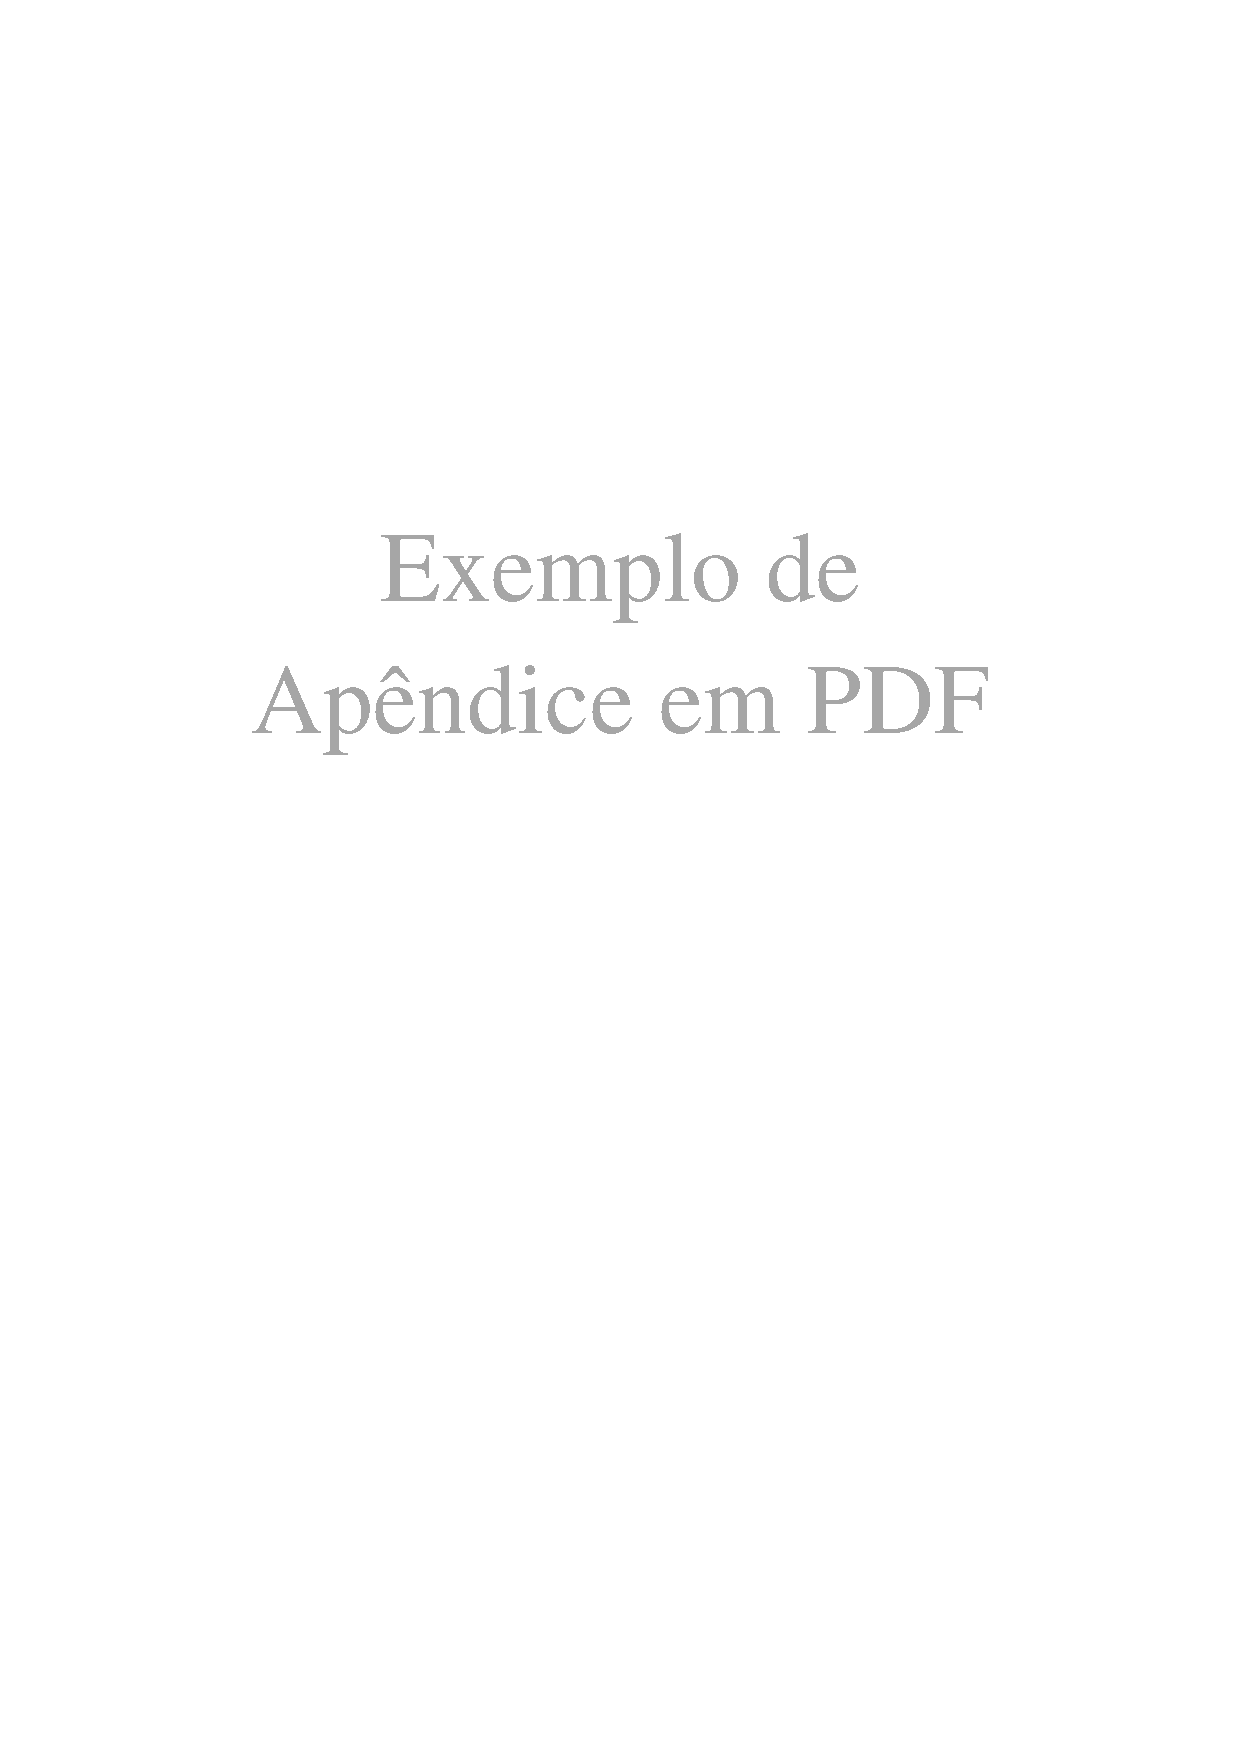
\includepdf[pages=-]{pdf_apendices/apendice_exemplo.pdf}
\end{apendicesenv}

\begin{anexosenv}


%-----------------------------Anexos-----------------------------%
% Imprime uma página indicando o início dos anexos

% ---
\chapter{Exemplo de anexo em pdf}
% ---
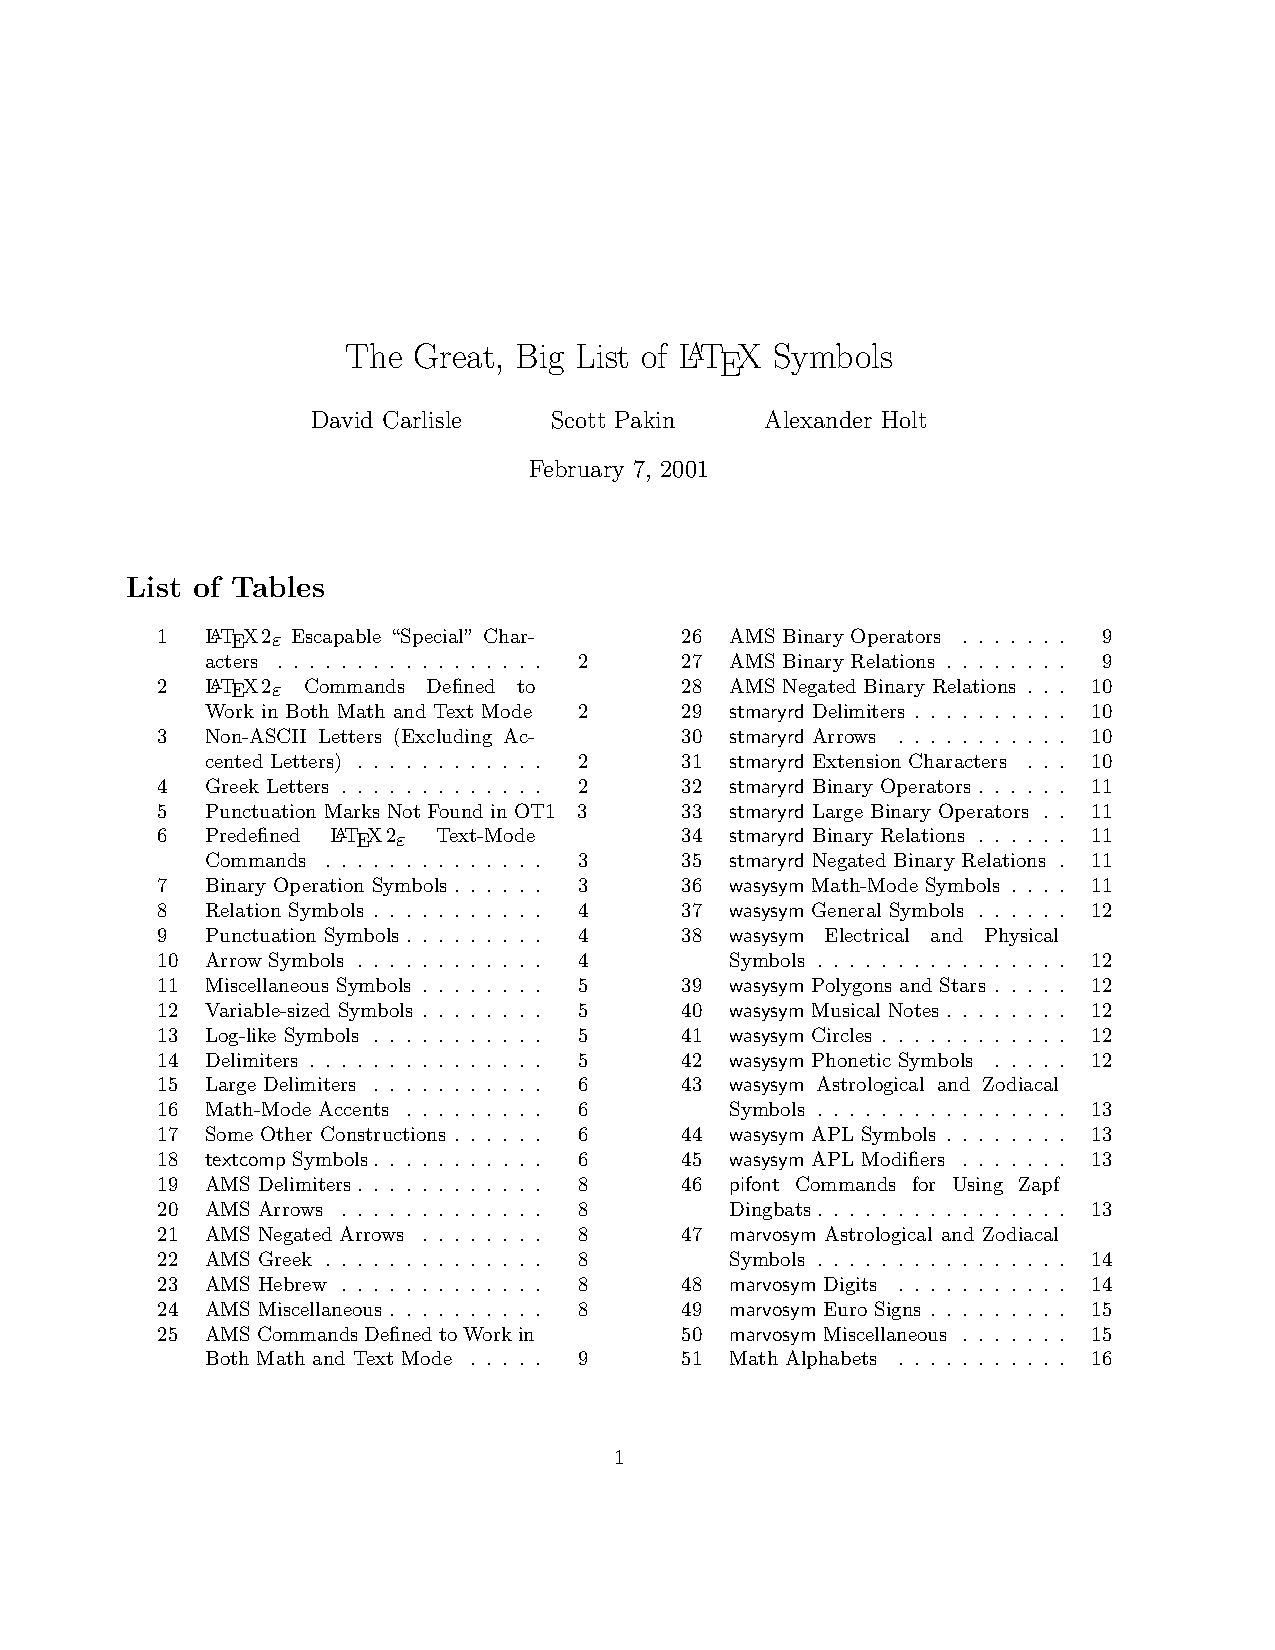
\includepdf[pages=-]{pdf_anexos/anexo_exemplo.pdf}
\end{anexosenv}
